\section{Framework of a centralized and decentralized system}
When looking at the traditional pyramid, which is fully centralized, it seems difficult, if not impossible to translate this to a decentralized solution as shown in \Cref{lit:manufacture}. It should be possible to determine whether a centralized or decentralized solution, using a MAS or holonic system, should be implemented at a business process. A framework to compare a centralized versus a decentralised solution is discussed here. Essential in the difference between these two possible solution spaces is the location of the processing power for the calculations. Centralised solutions have a single control unit where the information flows to, while decentralized solutions do not have this structure.

A popular comparison, discussed by \citet{parunak1999industrial}, is that of the original Roman army structures. Decisions where made at the top and dripped down, while the information stream went up. This method has been deployed in most companies. Due to the fact that something can be computed on a single computer, and be optimized on this single program, an optimal decision can be found.

However, the increasing complexity of computer and information systems, combined with the increasing complexity of their applications, exceed the level of conventional centralized computing. This is due to the processing of huge amounts of data, or data that originate from different locations. To solve such difficulties, computers have to act more like agents where each agent can solve, or decide on part of the problem. This is where agent-based architectures are an ideal fit to such a decentralized organizational structure.

To push the decision making to the lowest level, excessive layers of management can be obsolete. This allows for, sometimes, easier to understand and developing of problems, especially if the problem being solved is itself distributed.

By using principles of decomposition which is a classical optimization (reformulation) method \citep{sharif2012yard} presents a comparative study of two contrasting approaches for modelling the yard crane scheduling problem: centralized and decentralized. It seeks to assess their relative performances and factors that affect their performances. They conclude that a centralized approach outperforms the decentralized approach by 16.5 \% on average, due to having complete and accurate information about future truck arrivals. However, since the decentralized under performs the centralized, the decentralized approach can dynamically adapt to real-time dynamic changes, making it better suited for real-life operations. 

To optimize these different types of resources allocation problems, there are different kinds of allocation problems, for which different solutions are feasible. The purpose here is to find what characteristics are optimal to use a centralized vs a decentralized solution.


\subsection{Size and Modularity}
A critical aspect of the possibility to determine whether a centralized or decentralised solutions is preferred is the search space size of the problem. The size of the problem is seen as the number of resources or task that have to be allocated.  If a clear structure is conceivable and a clear population is in place a centralized solution is infeasible. This is due to the global overview. However, the high sensitivity to size and complexity makes a centralized solution impracticable.

In a decentralized structure, individual models are decoupled from one another, errors in one module impact only those modules that interact with it, leaving the rest of the system unaffected. This can be seen in \Cref{fig:modularitydecentral-changeability}. It shows however the importance of having a clear modular problem. 

\begin{figure}[h]
\centering
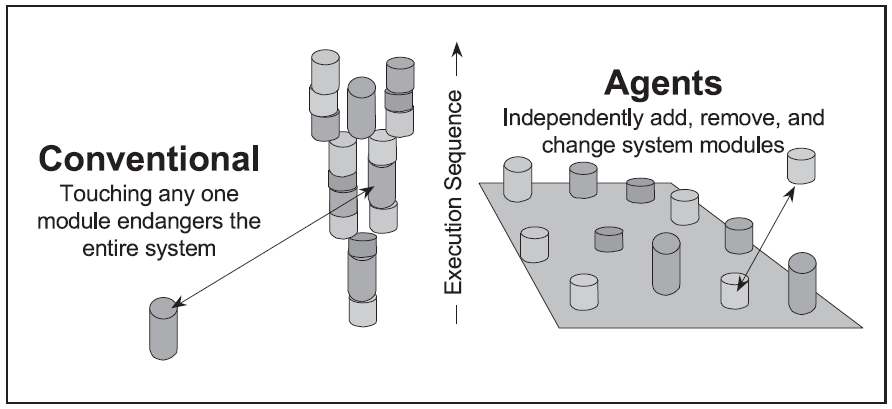
\includegraphics[width=0.7\linewidth]{img/modularity+decentral-changeability}
\caption{Comparison of a conventional control thread and an agent-based control, from \citep{parunak1999industrial}.}
\label{fig:modularitydecentral-changeability}
\end{figure}



\subsection{Dynamicity (Time Scale/Changeability)}
In a decentralized solution, the continuous monitoring of the state of the environment and typically the lack of complex decisions, a quick reaction to changes is possible. A high dynamical is the result. 

Unfortunately, it is difficult to achieve real-time scheduling in traditional manufacturing systems because the scheduling algorithms used are executed on a single, centralized computer that becomes computational incredibly difficult \citep{duffie1994real}.
\subsection{Solution Quality}
Since agent-based approaches are distributed, they do not have a global view of the entire state of a system. A lot can reached through communication and negotiation, but for a truly optimal solution, an entire view is necessary For example,  \citep{palmer2003decentralized} shows that this algorithm is not intended to find the optimal solution; it finds a good solution with less computation. 

In the centralized approach the assumption of a complete information on supply and demand is made. This requires rescheduling to adapt with changes. In the decentralized approach, no assumptions on the complete information is necessary. 


\subsection{Complexity}
Since an agent can execute actions only on its own surrounding, it is dependent on its local parameters. However, the agent can use information sent by its neighbours to adapt \citep{pujolle2006autonomic}. This interaction between the elements makes the complexity of a solution many times higher and more difficult than a centralized solution.

\subsection{Framework Overview}
Below a summary of the points above is given, with respect to the structure given. It is obvious that a decentralized solution is preferred, if the problem can be divided into sub problems. However, the real difficulty then lies in the complexity. Since in the system the communication becomes essential, the complexity increases.

\begin{tabular}{p{1.5cm} p{2.5cm} p{2.5cm} p{2.7cm}}
	\toprule
	& Centralised Solution & Decentralised Solution & Building Blocks\\
	\midrule
	Size / Modularity & Small; No sub-problems & Large; Ill-Structured; Easily dividable; Independent Modules & Population; Holonic; number of resources: (decision variables, parameters \& constraints) \citep{lang2015collaborative} \\
		\midrule
	Time scale and Changeability & Days - Weeks; Not subject to a lot of change & Real-time - Hour; Changeable  & Adaptive Capability ; Degree of Re- and Pro-activeness \citep{parunak1999industrial} \\
	\midrule
	Solution quality & Perfect & (sub-)Optimal & Object and Solution Space \citep{sharif2012yard} \\
	\midrule
	Complexity & Simple & Complex & Interaction between the set of elements; Communication \citep{pujolle2006autonomic} \\
	
	\bottomrule
\end{tabular}


\section*{Negotiation in a Decentralized Structure}
By decomposing the problem in smaller sub problems that a single agent can compute, and solve, the communication of the agents is essential. In order to integrate the solutions of the sub problems into the overall solution, the agents, which might not be cooperative, need to use negotiation.
%To achieve the autonomic-oriented architecture, we propose to select the appropriate control mechanisms among: 
%- adaptive: the agent adapts its actions according to the incoming events and to its vision of the current system state. The approach we propose is adaptive as the agent adapts the current control mechanisms and the actions undertaken when a certain event occurs. The actions the control mechanism executes may become no longer valid and must therefore be replaced by other actions. These new actions are indeed more suitable to the current observed state;
%- distribution: each agent is responsible for a local control. There is no centralization of the information collected by the different agents, and the decisions the agent performs are in no way based on global parameters. This feature is very important as this avoids having bottlenecks around a central control entity;
%- local: the agent executes actions on the elements of the node it belongs to. These actions depend on local parameters. However, the agent can use information sent by its neighbours to adapt the activated control mechanisms;
%- scalable: the proposed approach is scalable because it is based on a multi-agent system which scales well with the growing size of the controlled network. In order to adaptively control a new node, one has to integrate an agent (or a group of agents) in this node to perform the control. 
